\section{Implementation \& Evaluation}
\label{sec:eval}



\begin{table*}[t]
\centering
\begin{tabular}{clcl}
\hline
\multicolumn{1}{|l|}{\textbf{Rank}} & \multicolumn{1}{l|}{\textbf{Organization Name}}                  & \multicolumn{1}{l|}{\textbf{Rank}} & \multicolumn{1}{l|}{\textbf{Organization}}                     \\ \hline
\multicolumn{1}{|c|}{1}             & \multicolumn{1}{l|}{International Business Machines Corporation} & \multicolumn{1}{c|}{11}            & \multicolumn{1}{l|}{Hewlett Packard Company}                   \\ \hline
\multicolumn{1}{|c|}{2}             & \multicolumn{1}{l|}{Hitachi Ltd}                                 & \multicolumn{1}{c|}{12}            & \multicolumn{1}{l|}{Texas Instruments Incorporated}            \\ \hline
\multicolumn{1}{|c|}{3}             & \multicolumn{1}{l|}{Matsushita Electric Industrial Co Ltd,}      & \multicolumn{1}{c|}{13}            & \multicolumn{1}{l|}{Sony Corporation}                          \\ \hline
\multicolumn{1}{|c|}{4}             & \multicolumn{1}{l|}{Canon Kabushiki Kaisha,}                     & \multicolumn{1}{c|}{14}            & \multicolumn{1}{l|}{Intel Corporation}                         \\ \hline
\multicolumn{1}{|c|}{5}             & \multicolumn{1}{l|}{Motorola Inc,}                               & \multicolumn{1}{c|}{15}            & \multicolumn{1}{l|}{Micron Electric Co Ltd}                    \\ \hline
\multicolumn{1}{|c|}{6}             & \multicolumn{1}{l|}{Toshiba Corporation,}                        & \multicolumn{1}{c|}{16}            & \multicolumn{1}{l|}{Eastman Kodak Company}                     \\ \hline
\multicolumn{1}{|c|}{7}             & \multicolumn{1}{l|}{General Electric Company,}                   & \multicolumn{1}{c|}{17}            & \multicolumn{1}{l|}{Minnesota Mining \& Manufacturing Company} \\ \hline
\multicolumn{1}{|c|}{8}             & \multicolumn{1}{l|}{AT\&T Corp,}                                 & \multicolumn{1}{c|}{18}            & \multicolumn{1}{l|}{Microsoft Corporation}                     \\ \hline
\multicolumn{1}{|c|}{9}             & \multicolumn{1}{l|}{Fujitsu Limited,}                            & \multicolumn{1}{c|}{19}            & \multicolumn{1}{l|}{Samsung Electronics Co Ltd}                \\ \hline
\multicolumn{1}{|c|}{10}            & \multicolumn{1}{l|}{Xerox Corporation,}                          & \multicolumn{1}{c|}{20}            & \multicolumn{1}{l|}{NEC Corporation}                           \\ \hline                                                               
\end{tabular}
\caption{List of top 20 innovators for year 2013 as calculated by our proposed metrics.}
\label{lst:top20}
\end{table*}


\begin{table}[t]
		\begin{tabular}{| l | l |}
		\hline
		
		{Type} & {Count or Details} \\
		\hline
		\hline
		G1 Nodes & 1222689 \\
		G1 Edges & 3431064 \\
		G2 Nodes & 1222689 \\
		G2 Edges & 3431064 \\
		G1 Source Node & Kia Silverbrook \\
		Inventors with infinite dist. & \\
		Patents with zero citations & \\
		\hline
	\end{tabular}		
	\caption {\scriptsize Details of the co-authorship graph}
	\label{tab:model}
\end{table}	

\begin{table}[t]
	\begin{tabular}{| l | l |}
		\hline
		{Algorithm} & {Time (sec)} \\
		\hline
		\hline
		Bellman-Ford & 0.80 \\
		Dijkstra & 1.28 \\
		Johnson & 1.29 \\
		\hline
	\end{tabular}
	\caption {\scriptsize Performance of the three shortest path algorithms}
	\label{tab:algos}
\end{table}					

\begin{figure}[t]
  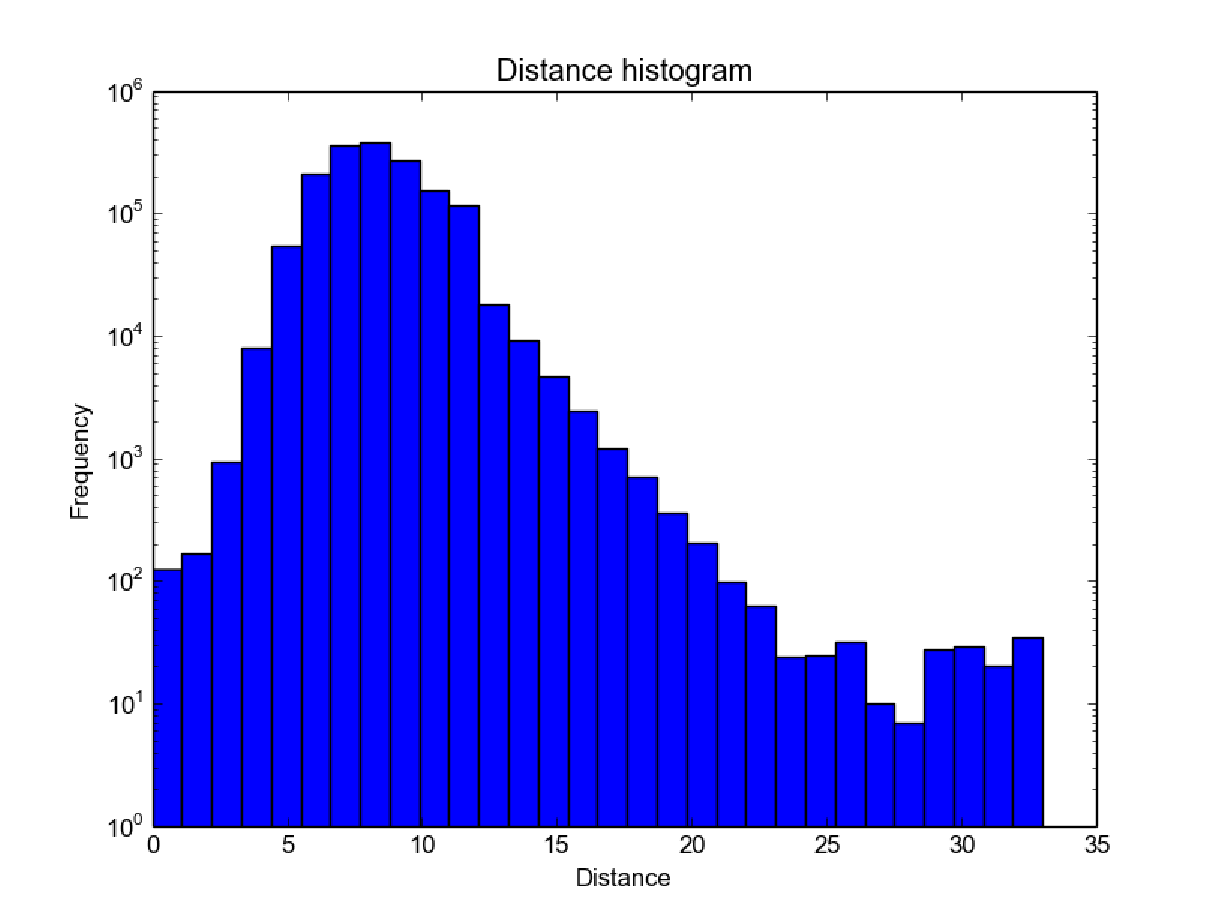
\includegraphics[scale=0.425]{figure/silver_brook_distance.pdf}
  \caption{\scriptsize Graph shows the frequency of nodes on Y-axis and the distance from
Kia Silverbrook on X-axis }
\label{fig:distance}
\end{figure}

\begin{figure}
  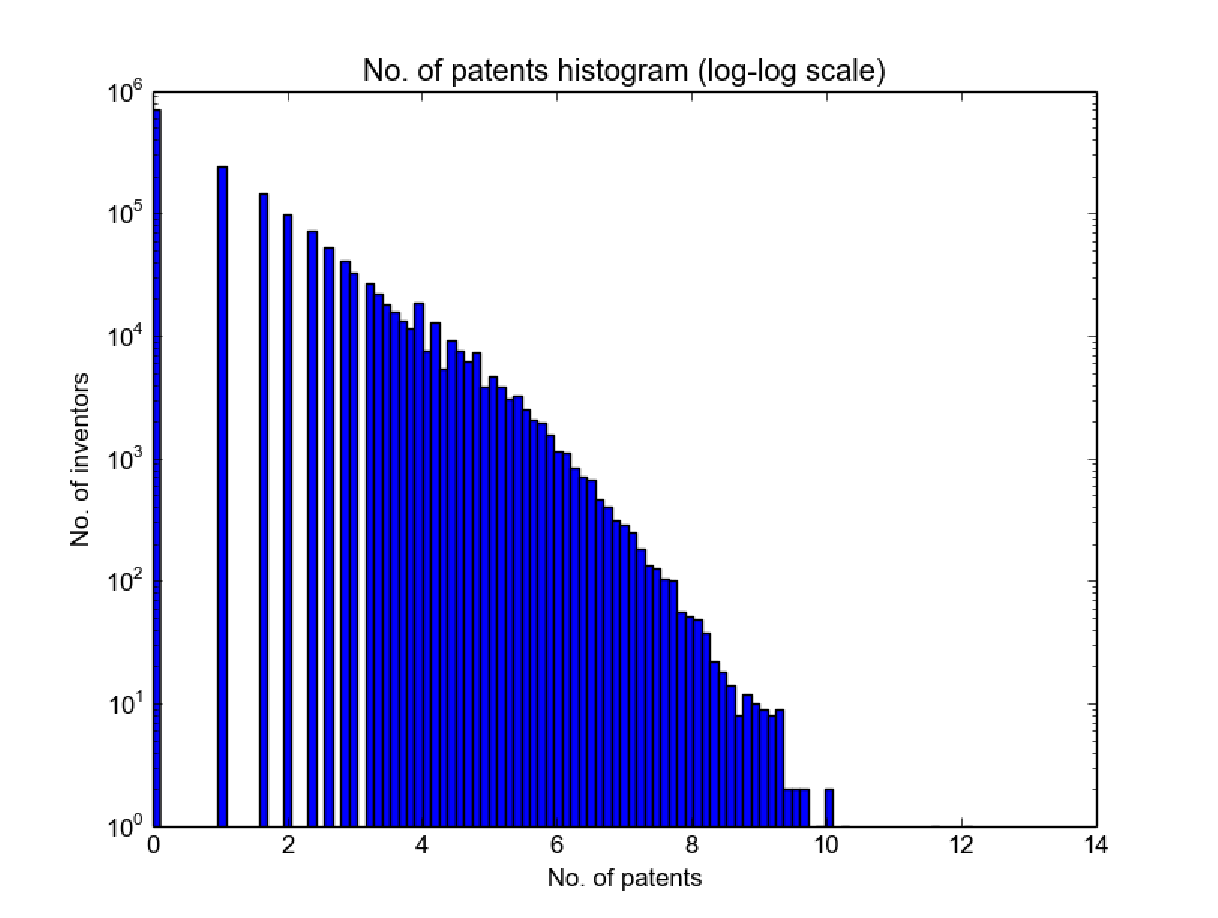
\includegraphics[scale=0.425]{figure/silver_log_log.pdf}
  \caption{\scriptsize Log-log scale graph of no. of patents on Y-axis and the no.of inventors on X-axis}
\label{fig:patent}	
\end{figure}

\begin{figure}[t]
  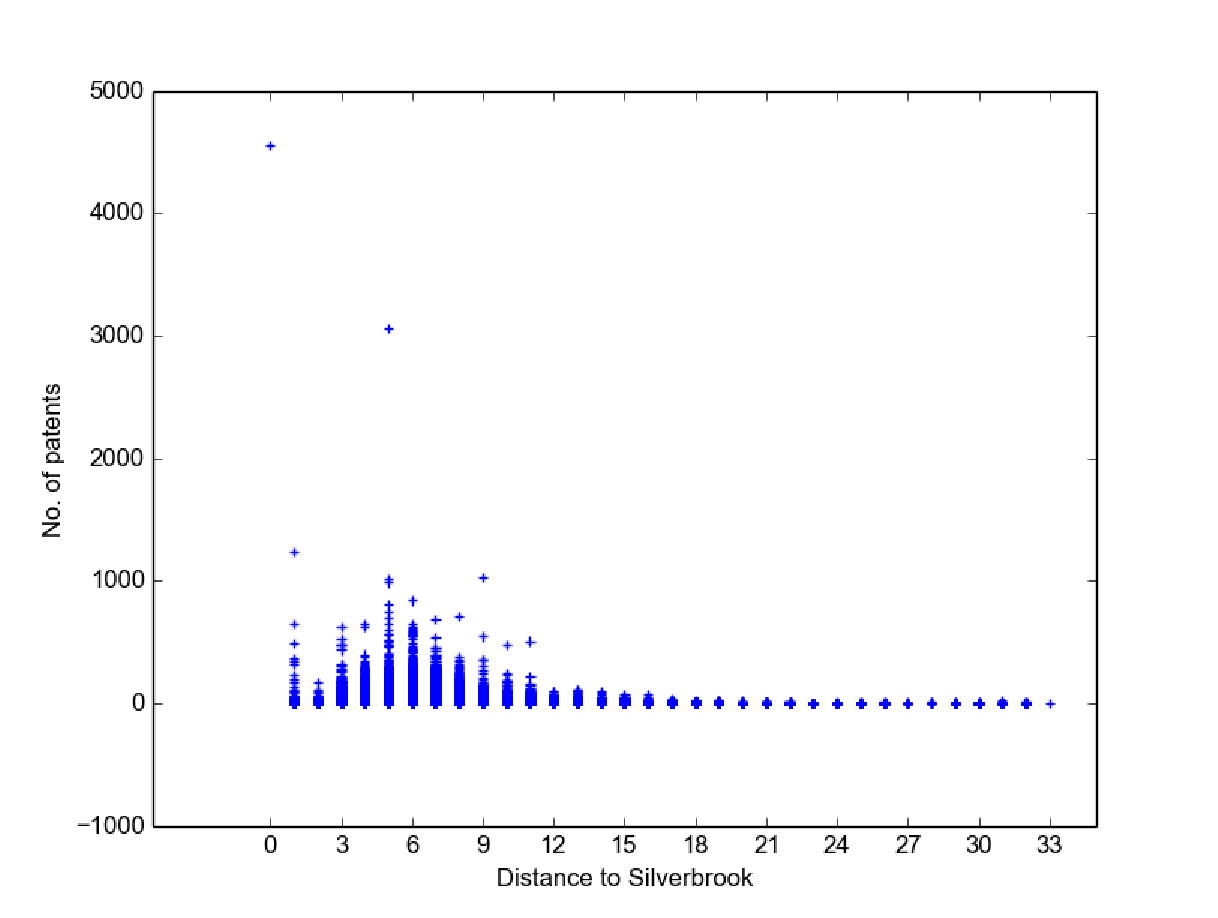
\includegraphics[scale=0.425]{figure/distance_patents.pdf}
  \caption{\scriptsize Relationship graph of no. of patents of an inventor and his distance from Kia Silverbrook}
\label{fig:distance_patent}
\end{figure}

\begin{figure}[t]
  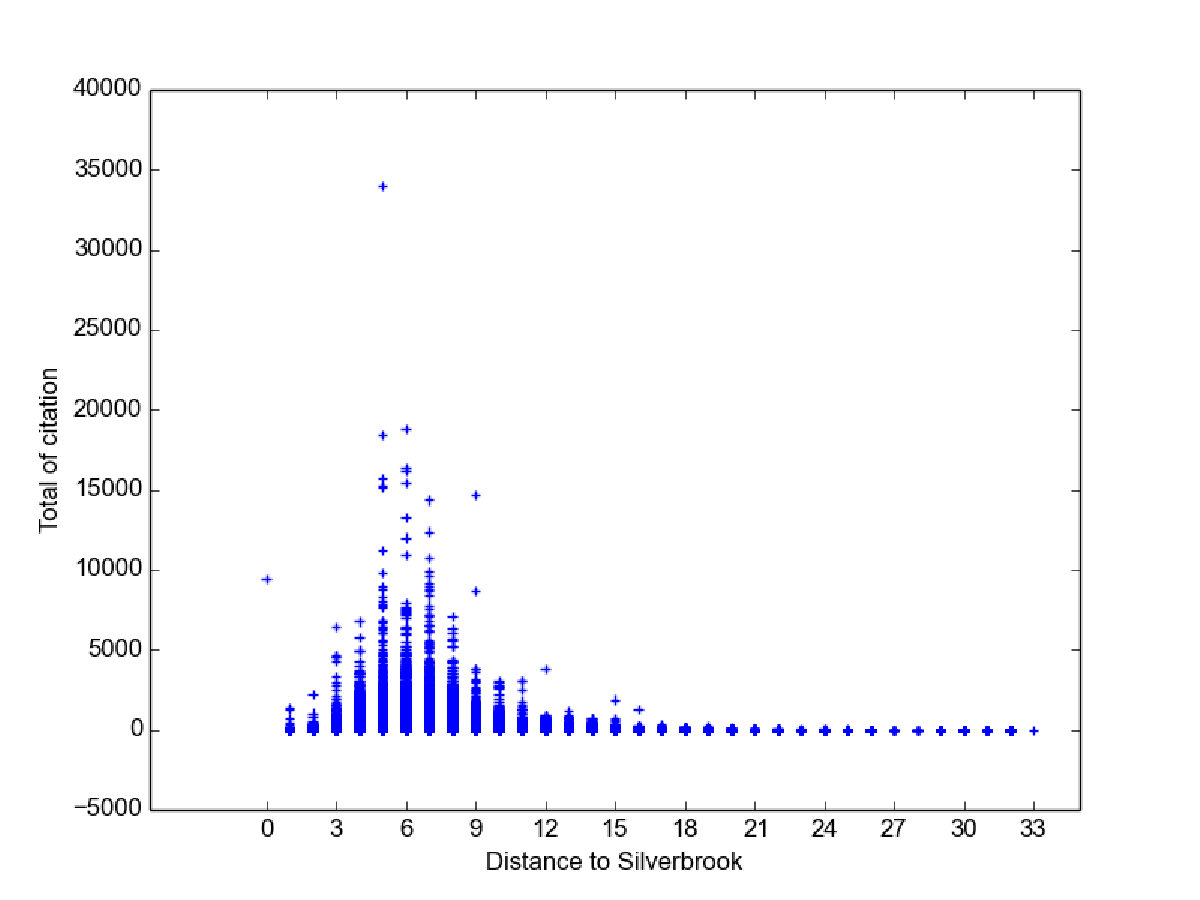
\includegraphics[scale=0.425]{figure/abc.pdf}
  \caption{\scriptsize Relationship graph of no. of citations for all patents of an inventor (i.e., the cumulative degree centrality) and his distance from Kia Silverbrook}
\label{fig:distance_citation}
\end{figure}



\begin{figure}[t]
  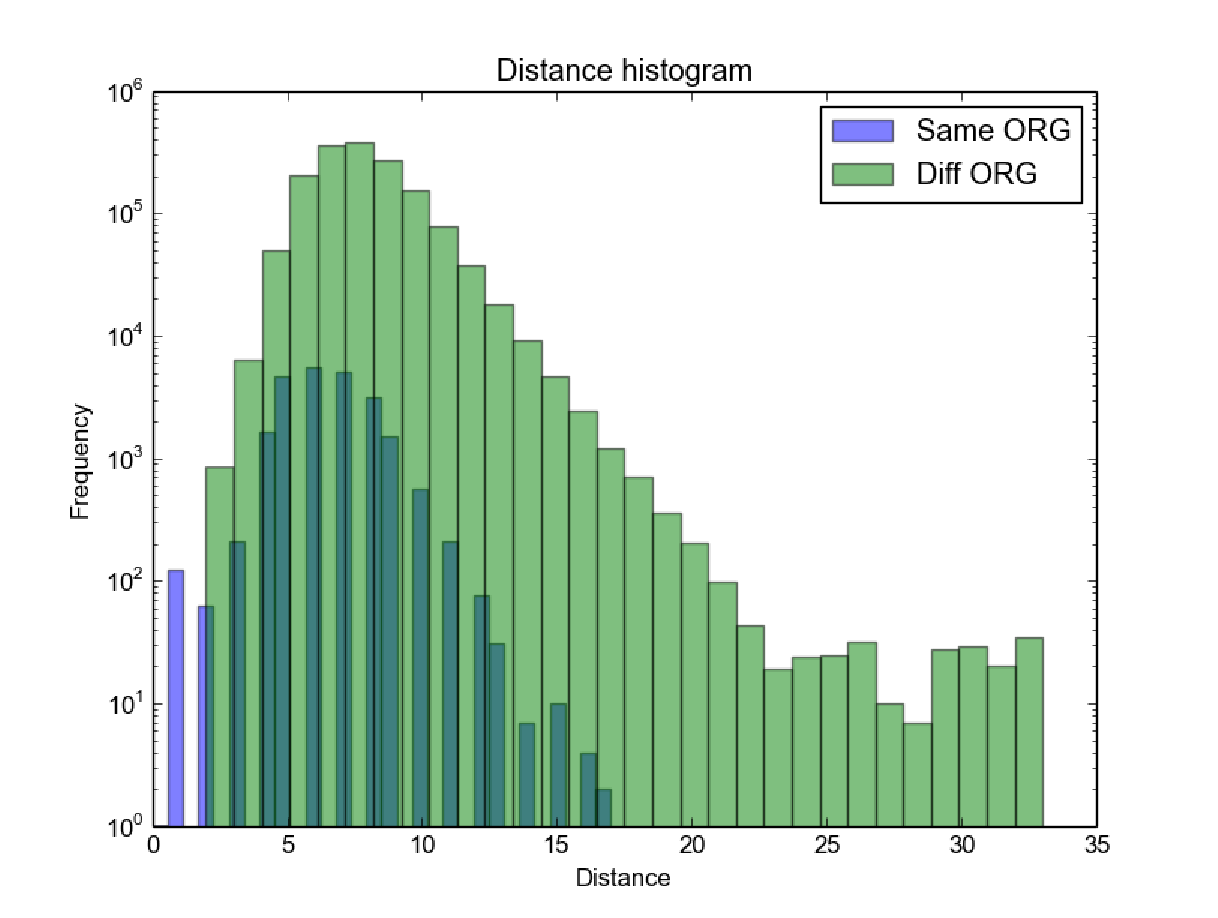
\includegraphics[scale=0.425]{figure/same_diff_org.pdf}
  \caption{\scriptsize Relationship graph of organisation of an inventor and his distance from Kia Silverbrook}
\label{fig:same_diff}
\end{figure}

We describe in detail our implementation method and evaluation procedure for
answering  our goals using the patent dataset. 

\subsection{Analysis Tools and Platform}


	\begin{itemize}
		\squish
		\item We use IGraph for all our graph analysis and metric
		calculation~\cite{gephi, igraph}. Table~\ref{tab:model} gives the details
		about Graph G1 in terms of its total number of nodes , edges , patents, the
		source node  of the graph and the average distance between the source node and
		all other nodes .    We choose Kia Silverbrook as our source node as he is one
		of the top and popular inventors in the patent dataset with maximum number of
		patents. We calculate the shortest path of all other nodes from Kia Silverbrook.
		We run three algorithms particularly Djikstra shortest path algorithm,
		Bellman-ford and Johnson available in IGraph tool on our Graph G1.
		\item The configuration of our experimental desktop machine is RAM $16$ GB, 12
		core with processor speed of $2.8$ GHz Intel i7 and platform is Ubuntu
		$14.04$.
	\end{itemize}

\subsection{Evaluation Steps}
	\begin{itemize}
		\squish
		\item {\em Evaluation Phase I - Collaborative Distance:} We calculated the 
		shortest path of each inventor w.r.t to Kia Silverbrook. We used three
		algorithms viz. Djikstra, Bellman-Ford, Johnson from IGraph to do this. We
		also analyzed their scalability with respect to the invention network graph
		and compared their performance.
		\item {\em Social Network Behavior:} Computed the distribution of the 
		collaborative distance w.r.t. Kia Silverbrook for our network, and also studied
		if the overall network follows power law for various popularity measures.
		\item {\em Evaluation Phase II - Degree centrality:} Use the in-built
		algorithm in IGraph to calculate degree centrality
		for each unique inventor and organization with respect to patents that cite his / her patent.
		\item {\em Data analysis and comparison:} Plot the graphs for the above
		generated data and analyze the relationship between the above two
		measurements. Compare our ranking results for the most innovative organization
		with publicly available list such as Reuters list, to check if our ranking
		metric coincides with the results of other metrics.
	\end{itemize}



\subsection{Results}
Table~\ref{tab:algos} shows the execution time for each of the three shortest
path algorithms  when run on our graph G1. We observe that Djikstra's
algorithm takes $1.28$ seconds, Bellman-ford takes $0.80$ seconds and Johnson
algorithm takes $1.29$ seconds to run on our experimental setup.
Figure~\ref{fig:distance} shows the result for the total number of inventors
having the same distance from Kia Silverbrook. This graph follows a normal
distribution. Figure~\ref{fig:patent} shows the log-log graph of the total
no.of patents to total no.of inventors. 


\paragraph{Question 1.}
Figure~\ref{fig:distance_patent} shows the relation of the distance from
Kia Silverbrook and the no. of patents for an inventor. This graph also follows a
normal distribution.

\paragraph{Question 2.}
To answer question Q2, we divide each inventor into either
or different organization. An inventor belongs to 
 same organization category if he has patent with any of the organizations that are 
assignees for Kia Silverbrook's patents. All other inventors fall in the different
organization category. With this division, we plot a graph as shown in Figure~\ref{same_diff}.
From the graph, we observe that inventors from same organization have
smaller collaborative distance which is expected. However, interesting observation is that
even many inventors from different organizations have smaller collaborative distance to Kia Silverbrook. 

\paragraph{Question 3.}


\subsection{Validation}

To validate the soundness of our proposed metrics, we cross-check our rankings
with public ally available rankings for the year 2013 by 24/7 Wall Street and
Reuters. These two lists are representatives of quantity and quality
respectively.  24/7 Wall Street report is purely based on number of patents
granted to an organization till that year.  On the other hand, Reuters
consider both quantitative as well as qualitative factors with respect to
time. Specifically, the factors such as volume of patents filed in last five
years, success ratio of filed patents, global contributions apart from US
patents, and citation impact of invention in last five years~\cite{reuters-method}.

Table~\ref{tab:validation} shows the top 5 innovative organizations in 2013 as
reported by 24/7 Wall Street and the corresponding rankings as per our
proposed metrics. We report that all of these 5 organizations occur in top 20
list as per our metrics (See Table~\ref{lst:top20} for the complete list).
This validates that our metric fairly succeeds in covering the quantitative
aspects of innovation.

We also compare our rankings to the list of top 100 innovators by Thomas
Reuters. Their report only states the top 100 innovators and does not give any
rankings. Thus, we only compare the percentage of organizations that fall in
top 100 in both Reuters are well as our rankings. On analysis, we find that
this intersection size is 41\%, which validates that our metric fairly
succeeds in covering the qualitative aspects of innovation.

\begin{table}[t]
\centering
\begin{tabular}{|l|c|c|}
\hline
\textbf{Organization}        & \multicolumn{1}{l|}{\textbf{24/7 Wall St}} & \multicolumn{1}{l|}{\textbf{SSL 3.0}} \\ \hline
IBM Corp                     & 1                                          & 1                                         \\ \hline
Samsung Electronics          & 2                                          & 19                                        \\ \hline
Canon K K                    & 3                                          & 4                                         \\ \hline
Sony Corp                    & 4                                          & 13                                        \\ \hline
Microsoft Corp               & 5                                          & 18                                        \\ \hline
\end{tabular}
\caption{Comparison of Rankings by 24/7 Wall St vs. SSL 3.0.}
\label{tab:validation}
\end{table}

% References:
% http://www.forbes.com/innovative-companies/
% http://top100innovators.com/
% http://www.brw.com.au/lists/50-most-innovative-companies/2014/
